\documentclass{report}
\usepackage{graphicx}
\usepackage{caption}
\usepackage{verbatim}
\usepackage{listings}

\begin{document}

 \begin{center}

   
\includegraphics[width=0.4\textwidth]{gubcse.png}   
   \vspace{0.5cm}    \\
   {\LARGE\textbf{Green University of Bangladesh}}     \\
   \vspace{0.5cm}
   {\Large Department of Computer Science and engineering}
       \rule{\linewidth}{0.5mm}   \\
       \vspace{0.5cm}
       {\Large \textbf{Lab Report -03}}   \\
       \vspace{0.5cm}
       {\Large\textbf{Course title : } Object Oriented Programming Lab   \\
       {\Large Course Code: CSE-221              }
         {\Large Section: DA  } \\
              \vspace{0.5cm}

       {\Large\textbf{Experiment title : } Box Volume Calculator Program in Java     \\
              \vspace{0.5cm}
    \rule\linewidth{0.5mm}
     {\Large Semester: Spring, Year: 2023         Program: B.Sc in CSE (Day)}    \\
     \vspace{0.3cm}
      {\Large submitted by }    \\
      \vspace{0.3cm}
     {\LARGE\textbf{  IBRAHIM REFAT}}   \\
     {\LARGE\textbf{ ID: 221902333}}
              \vspace{0.5cm}

         \Large  Lab Date: 06/03/2023    \\
         \Large Submission Date: 12/03/2023    \\
         \Large Course Teacher: Dr. Muhammad Aminur Rahaman

       
 \end{center}

\clearpage


\section{Title}
\Large Implement Box volume calculator

\section{Objective }
\begin{enumerate}
\item  Create a class Box having three private variables length, width, and height. \\
\item  Construct three constructors into the Box class. 1st constructor will be the default constructor, 2nd will be designed for accepting three values of length, width, and height. 3rd will be designed for accepting any object of the Box class.   \\
\item . Design a display() method to print the volume of the box which will be called from the main method of the Main class by creating 3 objects using the three constructors.

\section{Procedure}
\begin{enumerate}
\item  Create a Class called "BoxConstructor".

\item  Within this class, declare three private 
variables: "length", "width", and "height",
 all of which are of type double.

\item Create a default public constructor  Within this constructor,
 set the values of "length", "width", and "height"


\item Create another public constructor for the class "BoxConstructor" that accepts three parameters:
 "length", "width", and "height". Within this constructor, set the values of "length", "width", and "height" to the values passed in as parameters.

\item Create another constructor for the class "BoxConstructor" that calculates the volume 
of the box and prints it to the console. Within this constructor, use the 
formula "length * width * height" to calculate the volume of the box, then print the result to the console.

\item  In the main method of the program, create a Scanner object to read user input.
\item  Create an instance of the "BoxConstructor" class called "defaultBox" using the default constructor.

\item Prompt the user to enter the values for "length", "width", and "height" of the box using the Scanner object.

\item  Create an instance of the "BoxConstructor" class called "valueAcceptingBox" using the
 constructor that accepts three parameters, passing in the values entered by the user.


\item Call the "BoxVolume()" method on the "valueAcceptingBox" instance to calculate the volume of the box.

\item  Print the volume of the box to the console.



\end{enumerate}

\section{Implementation}
\begin{lstlisting}[language=Java, breaklines=true]
    /*
author IBRAHIM REFAT
ID : 221902333
*/
import java.util.Scanner;
public class BoxConstructor {
    
     private double length;
    private double width;
    private double height;
    
    public BoxConstructor() {
        length = 0;
        width = 0;
        height = 0;
    }
    
    public BoxConstructor(double length, double width, double height) {
        this.length = length;
        this.width = width;
        this.height = height;
    }
    
    public double BoxVolume() {
        return length * width * height;
    }
    
    public static void main(String[] args) {
        Scanner scan = new Scanner(System.in);
        
        BoxConstructor defaultBox = new BoxConstructor();
        
        System.out.print("Enter length of Box : ");
        double length = scan.nextDouble();
        System.out.print("Enter width of Box : ");
        double width = scan.nextDouble();
        System.out.print("Enter height of Box : ");
        double height = scan.nextDouble();
        
        BoxConstructor valueAcceptingBox = new BoxConstructor(length, width, height);
        double volume = valueAcceptingBox.BoxVolume();
        System.out.println("Volume of the box is: " + volume);
    }
    
}

\end{lstlisting}

\section{ Test Result}
\centering 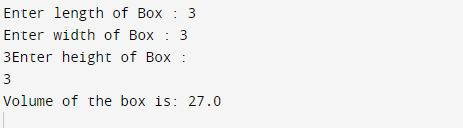
\includegraphics[width=1.2\textwidth]{output.JPG}
\cerntering  Figure : 01 
\section{ANALYSIS AND DISCUSSION}
\begin{verbatim}
    From this code, we can learn how to create a java class 
    that represents a three dimensional box object and 
    provides constructros and method to initialize and 
    manipulate the object. and we learn from this  
    how method in java class calculate and return the volume
    of box. In Java programming, we consider everything 
    to be an object. For example, a box can be represented
    as an object with three parameters: length, width, 
    and height. These parameters help us visualize the 
    appearance of the box.
\end{verbatim}

\end{document}
